\documentclass[paper=a4,UTF8,fontsize=11pt]{scrartcl} % A4 paper and 11pt font size
\usepackage[noend]{algpseudocode}
\usepackage{ctex}
\usepackage[T1]{fontenc} % Use 8-bit encoding that has 256 glyphs
\usepackage{fourier} % Use the Adobe Utopia font for the document - comment this line to return to the LaTeX default
\usepackage[english]{babel} % English language/hyphenation
\usepackage{amsmath,amsfonts,amsthm} % Math packages
\usepackage[english]{babel}
\usepackage[utf8]{inputenc}
\usepackage{indentfirst}
\usepackage{algorithm}
\usepackage{lipsum} % Used for inserting dummy 'Lorem ipsum' text into the template
\usepackage{float}
\usepackage{sectsty} % Allows customizing section commands
\allsectionsfont{\centering \normalfont\scshape} % Make all sections centered, the default font and smaıll caps
\usepackage{graphicx}
\usepackage{fancyhdr} % Custom headers and footers
\pagestyle{fancyplain} % Makes all pages in the document conform to the custom headers and footers
\fancyhead{} % No page header - if you want one, create it in the same way as the footers below
\fancyfoot[L]{} % Empty left footer
\fancyfoot[C]{\thepage} % Empty center footer
\fancyfoot[R]{} % Page numbering for right footer
\renewcommand{\headrulewidth}{0pt} % Remove header underlines
\renewcommand{\footrulewidth}{0pt} % Remove footer underlines
\setlength{\headheight}{13.6pt} % Customize the height of the header
\usepackage[noend]{algpseudocode}
\numberwithin{equation}{section} % Number equations within sections (i.e. 1.1, 1.2, 2.1, 2.2 instead of 1, 2, 3, 4)
\numberwithin{figure}{section} % Number figures within sections (i.e. 1.1, 1.2, 2.1, 2.2 instead of 1, 2, 3, 4)
\numberwithin{table}{section} % Number tables within sections (i.e. 1.1, 1.2, 2.1, 2.2 instead of 1, 2, 3, 4)
\usepackage{color}
\setlength\parindent{0.3pt} % Removes all indentation from paragraphs - comment this line for an assignment with lots of text
\usepackage{graphicx}
\usepackage{xcolor}
\usepackage{listings}
\definecolor{mygreen}{rgb}{0,0.6,0}
\definecolor{mygray}{rgb}{0.5,0.5,0.5}
\definecolor{mymauve}{rgb}{0.58,0,0.82}

\lstset{ 
  language=C++,
  backgroundcolor=\color{white},   % choose the background color
  basicstyle=\footnotesize,        % size of fonts used for the code
  breaklines=true,                 % automatic line breaking only at whitespace
  captionpos=b,                    % sets the caption-position to bottom
  commentstyle=\color{mygreen},    % comment style
  escapeinside={\%*}{*)},          % if you want to add LaTeX within your code
  keywordstyle=\color{blue},       % keyword style
  stringstyle=\color{mymauve},     % string literal style
}
% \lstset{language=C++,
%                 basicstyle=\ttfamily,
%                 keywordstyle=\color{blue}\ttfamily,
%                 stringstyle=\color{red}\ttfamily,
%                 commentstyle=\color{green}\ttfamily,
%                 morecomment=[l][\color{magenta}]{\#}
% }



%----------------------------------------------------------------------------------------
%	TITLE SECTION
%----------------------------------------------------------------------------------------

\newcommand{\horrule}[1]{\rule{\linewidth}{#1}} % Create horizontal rule command with 1 argument of height
\title{
\normalfont \normalsize
\textsc{Shanghai Jiao Tong University} \\ [25pt] % Your university, school and/or department name(s)
\horrule{0.5pt} \\[0.4cm] % Thin top horizontal rule
\huge \kaishu 哈希表设计 \\ % The assignment title
\horrule{2pt} \\[0.5cm] % Thick bottom horizontal rule
}

\author{\\ \kaishu 吕艺\\ \normalsize 517021910745} % Your name

\date{\normalsize\today} % Today's date or a custom date

\begin{document}

\maketitle % Print the title
\kaishu
\section{需求分析}

1.本演示文件的主要需求建立哈希表。具体背景为对文件读入的30个人名建立哈希表,进行必要的查表和建表功能。要实现的具体功能有建立哈希表,通过学生的名字查找哈希表,在哈希表中对指定学生作删除标记,以及彻底删去做了了删除标记的学生。
\vspace{0.5cm}

2.演示文件无需用户输入,程序自动将哈希表中的学生按名字排序后打印学生的名字
\vspace{0.5cm}

3.程序执行的命令包括:

a.根据除留余数法将学生放在哈希表的不同位置,并通过线性探测法解决冲突

b.按顺序打印哈希表中学生的名字

c.将学生插入到哈希表中

d.在哈希表中对指定学生作删除标记

e.彻底删去做了删除标记的学生

\vspace{0.5cm}
4.测试数据

演示文件中用到的测试数据为文件读入的30个中文人名拼音,长度不超过20个字符。
\vspace{0.8cm}

\section{概要设计}

本演示文件中的哈希表采用的是除留取余的哈希函数,以及线性探测法的冲突解决方法。为了实现这一功能,演示文件中定义了$student$结构体,父类$hashTable$,以及派生类$closeHashTable$

1)结构体 $student$

数据对象: char * name = NULL;\ \ \ \ \ \ \ \ \ \ \quad int state;

基本操作:student(){state = 0;}

\qquad \qquad \quad \ \ \ 操作条件: $student$还未被初始化

\qquad \qquad \quad \ \ \ 操作结果: 默认构造$student$类的对象

\qquad \qquad \quad \ \ \     student(char * names) {name = names; state = 0;}

\qquad \qquad \quad \ \ \ 初始条件:	$student$类还未被初始化

\qquad \qquad \quad \ \ \ 操作结果:根据名字初始化$student$类的对象

\qquad \qquad \quad \ \ \ char * getName() const \{return name;\}

\qquad \qquad \quad \ \ \ 初始条件:$student$类已经被初始化

\qquad \qquad \quad \ \ \ 操作结果: 返回$student$类的实例对象的名字

\qquad \qquad \quad \ \ \      int getState () const{return state;}

\qquad \qquad \quad \ \ \  操作条件: $student$类已被初始化

\qquad \qquad \quad \ \ \ 操作结果: 返回$student$类的实例对象的状态

\qquad \qquad \quad \ \ \ void changeState(int state1){state = state1;}

\qquad \qquad \quad \ \ \ 操作条件:$student$类已经被初始化 

\qquad \qquad \quad \ \ \ 操作结果:返回$student$类的实例对象的状态改变为$state1$

\qquad \qquad \quad \ \ \     void setName( char* c)	{name = c;}

\qquad \qquad \quad \ \ \ 操作条件: $student$类被初始化 

\qquad \qquad \quad \ \ \ 操作结果: 给$student$类的对象设置名字
\vspace{0.2cm}

2)父类 $hashTable$

基本操作:virtual bool find(const Type \& x) const= 0;

\qquad \qquad \quad \ \ \   virtual bool insert(const Type \& x) = 0;

\qquad \qquad \quad \ \ \ char * getName() const \{return name;\}

\qquad \qquad \quad \ \ \      virtual bool remove(const Type \& x) = 0;
\vspace{0.2cm}

3)派生类$closeHashTable$

数据对象: student * array;\ \ \ \ \ \ \ \ \ \ \qquad     int size;

 \qquad \qquad \ \ \ \ \ \ \  int(*key)(const Type x);

基本操作:closeHashTable(int length, int(*f)(const Type x));

\qquad \qquad \quad \ \ \ 操作条件: $closeHashTable$还未被初始化

\qquad \qquad \quad \ \ \ 操作结果: 根据哈希函数将学生插入到哈希表的特定位置

\qquad \qquad \quad \ \ \ bool insert(const Type \& x);

\qquad \qquad \quad \ \ \ 初始条件:	$closeHashTable$类已被初始化

\qquad \qquad \quad \ \ \ 操作结果:将该学生插入到指定位置

\qquad \qquad \quad \ \ \    bool remove(const Type \& x);

\qquad \qquad \quad \ \ \ 初始条件:$closeHashTable$类已经被初始化

\qquad \qquad \quad \ \ \ 操作结果: 在哈希表中对指定学生作删除标记

\qquad \qquad \quad \ \ \     bool find(const Type \& x) const;

\qquad \qquad \quad \ \ \  操作条件: $closeHashTable$类已被初始化

\qquad \qquad \quad \ \ \ 操作结果: 返回指定学生是否在该表中存在的布尔值

\qquad \qquad \quad \ \ \ void changeState(int state1){state = state1;}

\qquad \qquad \quad \ \ \ 操作条件:$student$类已经被初始化 

\qquad \qquad \quad \ \ \ 操作结果:返回$student$类的实例对象的状态改变为$state1$

\qquad \qquad \quad \ \ \ void rehash();

\qquad \qquad \quad \ \ \ 操作条件: $closeHashTable$类已被初始化 

\qquad \qquad \quad \ \ \ 操作结果: 彻底删除哈希表中做了删除标记的学生

\vspace{0.3cm}

2.本程序包括两个模块:

1)  主函数模块

\qquad int main() \{

    \qquad \quad ifstream in;
    
    \qquad \quad in.open("name.txt");
    
    \qquad \quad int (*f)(const student A) = hash1;
    
    \qquad \quad closeHashTable<student> a(30, f);
    
    \qquad \quad char tmp[Num][20];
    
    \qquad \quad for(int i = 0;i < Num; i++)\{
    
    \qquad \quad in >> tmp[i];
        
    \qquad \quad student A = student(tmp[i]);
        
    \qquad \quad a.insert(A);\} 
    
    \qquad \quad for(int i = 0 ; i< 30 ; i++)
    
    \qquad \qquad \ \ \ \ if (a.array[i].getState() == 1) 
        
    \qquad \qquad \ \ \ \ \{ cout << a.array[i].getName() << endl; \}
    
    \qquad \quad    return 0;
\}
       
2)  父类$hashTable$单元模块--定义派生类必须实现的功能

3)派生类$closeHashTable$单元模块--具体实现功能

\section{详细设计}
1)$hashTable$单元模块
\lstinputlisting{father.h}

2)$closeHashTable$单元模块
\lstinputlisting{11.cpp}

3)主函数模块
\lstinputlisting{mainn.cpp}

\vspace{0.3cm}
\section{调试分析}
1.一开始本演示文件仅设计了$closeHashTable$类,将所有操作都直接定义在了这个类中,这导致程序的可移植性较低,为了更好地规范哈希表的基本操作,程序中又设计了$hashTable$父类,将$closeHashTable$类作为$hashTable$类的派生类,规范了哈希表的基本操作。
\newpage
2.算法的复杂度分析

1)时间复杂度
由于采用数组的形式存储学生的名字,各种操作的算法复杂度比较合理。
$closeHashTable$类的构造函数的时间复杂度是$O(1)$, 函数$insert$,$remove$,$find$,$rehash$的时间复杂度均为$O(n)$。

$closeHashTable$类的初始化函数仅将学生个数,名字矩阵和指向哈希函数的函数指针赋值,因此这个函数的时间复杂度为$O(1)$。

$insert$,$remove$,$find$和$rehash$函数的时间复杂度都与元素个数成正比,因此时间复杂度为$O(n)$。

2)空间复杂度

$closeHashTable$类模块的空间复杂度与叶节点的个数成正比,即$O(n)$。
主函数模块的复杂度取决于定义主函数作用域中的$closeHashTable$类,故空间复杂度也为$O(n)$。
\vspace{0.2cm}

\section{用户手册}
1.本程序以Jetbrains Clion 2018.2.5, 采用C++ 11 标准,程序以项目方式组织(project),如图1所示:
\begin{figure}[h]
    \centering
    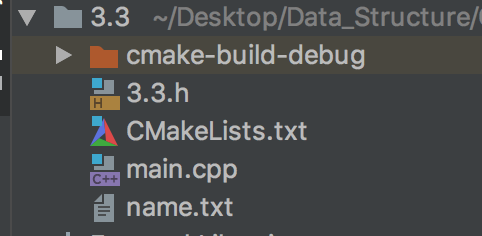
\includegraphics[width=0.5\textwidth]{33.png}
\end{figure}

2.依次点击菜单"Run"->build,再点击"Run",程序就执行哈希表的生成,并按哈希表的顺序打印对应学生的名字
\begin{figure}[h]
    \centering
    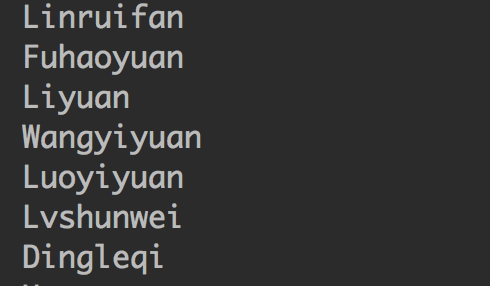
\includegraphics[width=0.5\textwidth]{result1.png}
\end{figure}

\section{测试结果}
程序开始后读入"name.txt"中的30个学生的名字,并根据哈希函数对他们进行排序并将排序后的学生名字依次打印在屏幕上。

\section{附录}

源程序文件名清单

main.cpp               \qquad \quad  //主函数

hashTable.h            \qquad //哈希表单位模块



\end{document}




